\documentclass[xcolor=svgnames]{beamer}
\usepackage[utf8]{inputenc}
\usepackage[T1]{fontenc}
\usepackage{xcolor}
\usepackage{booktabs}
\usepackage{amsmath}
\usepackage{graphicx}
\usepackage{siunitx} % For SI units
\usepackage{hyperref}
\usetheme{Madrid}

% COLORS and FOOTNOTE settings (copy from previous file)
\definecolor{mqred}{RGB}{166, 25, 46}
\definecolor{mqdeepred}{RGB}{118, 35, 47}
\definecolor{mqgray}{RGB}{55, 58, 54}
\definecolor{mqlightgray}{RGB}{237, 235, 229}
\definecolor{mqmagenta}{RGB}{198, 0, 126}
\usecolortheme[named=mqred]{structure}
\setbeamercolor{title in head/foot}{bg=mqlightgray, fg=mqgray}
\setbeamercolor{author in head/foot}{bg=mqdeepred}
\setbeamercolor{page number in head/foot}{bg=mqdeepred, fg=mqlightgray}
\makeatletter
\setbeamertemplate{footline}{
  \leavevmode%
  \hbox{%
  \begin{beamercolorbox}[wd=.5\paperwidth,ht=2.25ex,dp=1ex,center]{author in head/foot}%
    \usebeamerfont{author in head/foot}\insertshortauthor\expandafter\ifblank\expandafter{\beamer@shortinstitute}{}{~~(\insertshortinstitute)}
  \end{beamercolorbox}%
  \begin{beamercolorbox}[wd=.4\paperwidth,ht=2.25ex,dp=1ex,center]{title in head/foot}%
    \usebeamerfont{title in head/foot}\insertshorttitle
  \end{beamercolorbox}%
  \begin{beamercolorbox}[wd=.1\paperwidth,ht=2.25ex,dp=1ex,center]{page number in head/foot}%
    \usebeamerfont{page number in head/foot}\insertframenumber{} / \inserttotalframenumber
  \end{beamercolorbox}}%
  \vskip0pt%
}
\makeatother
\beamertemplatenavigationsymbolsempty


% TITLE, AUTHORS, INSTITUTE, DATE
\title[Thermo: Quantifying Heat]{Thermodynamics Lesson 2: Quantifying Heat and Changing States}
\author[P. Haynes]{Mr Haynes}
\institute[GHS]{Gosford High School}
\date{\today}

% LOGO (Optional)
%\titlegraphic{\includegraphics[height=2.5cm]{logo.jpg}}

\begin{document}

\begin{frame}
    \titlepage
\end{frame}

\begin{frame}{Outline}
    \tableofcontents
\end{frame}

\section{Review}
\begin{frame}{Review Lesson 1}
    \frametitle{Recap: Temperature and Heat Transfer}
    \begin{itemize}
        \item Temperature measures average particle KE [N1].
        \item Heat is energy transferred due to $\Delta T$.
        \item Mechanisms: Conduction, Convection, Radiation [N4].
    \end{itemize}
    \vspace{1em}
    \textbf{Think/Pair/Share:} Why does beach sand get much hotter than ocean water under the same sunlight?
    \pause
    \begin{itemize}
        \item \textit{Answer Hint:} Different substances require different amounts of energy to change temperature by the same amount.
    \end{itemize}
\end{frame}

\section{Specific Heat Capacity}
\begin{frame}{Specific Heat Capacity (c) [N3]}
    \frametitle{Heating Up: Specific Heat Capacity}
    \begin{itemize}
        \item \textbf{Definition:} The amount of heat energy required to raise the temperature of \textbf{1 kg} of a substance by \textbf{1 K} (or 1 °C).
        \item Symbol: $c$
        \item Units: \si{J.kg^{-1}.K^{-1}} or \si{J.kg^{-1}.\celsius^{-1}}
        \item \textbf{High 'c'} (like water: $\approx 4186$): Takes a LOT of energy to heat up (and stores a lot).
        \item \textbf{Low 'c'} (like sand/metals: $\approx 800$/$400$): Heats up quickly with less energy.
        \item \textbf{Formula:} The heat energy ($Q$) needed for a temperature change ($\Delta T$) depends on mass ($m$) and specific heat capacity ($c$):
        \begin{equation*}
        \alert{Q = mc\Delta T}
        \end{equation*}
        where $\Delta T = T_{final} - T_{initial}$.
    \end{itemize}
\end{frame}

\section{Latent Heat}
\begin{frame}{Changing State: Latent Heat (L) [N5]}
    \frametitle{Energy for Phase Changes: Latent Heat}
    \textbf{Observation (Heating Curve):} When a substance melts or boils, its temperature \textit{remains constant} even though heat is being added.
    \vspace{1em}
    \textbf{Why?}
    \begin{itemize}
        \item Energy is used to overcome intermolecular forces (increase potential energy), not increase kinetic energy (temperature).
    \end{itemize}
    \vspace{1em}
    \textbf{Definition:} Latent heat ($L$) is the energy absorbed or released per unit mass during a phase change at constant temperature.
    \begin{itemize}
        \item \textbf{Latent Heat of Fusion ($L_f$):} Energy for solid $\leftrightarrow$ liquid change.
        \item \textbf{Latent Heat of Vaporization ($L_v$):} Energy for liquid $\leftrightarrow$ gas change. (Typically $L_v > L_f$)
    \end{itemize}
    \textbf{Formula:} Heat energy ($Q$) for phase change of mass ($m$):
    \begin{equation*}
    \alert{Q = mL}
    \end{equation*}
    (Use $L_f$ for melting/freezing, $L_v$ for boiling/condensing)
\end{frame}

\section{Heating Curves}
\begin{frame}{Analysing Heating Curves [N5 Analyse]}
    \frametitle{Putting It Together: The Heating Curve}
    \begin{center}
    % Placeholder - insert graph image
    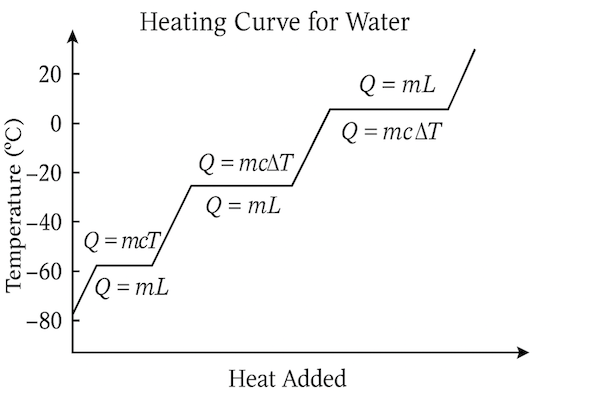
\includegraphics[width=0.4\textwidth]{img/water_heating.png}

    \textit{Temperature vs Energy Added for Water}
    \end{center}
    \begin{itemize}
        \item \textbf{Sloped Sections:} Temperature changes. Energy increases particle KE. Use $Q=mc\Delta T$. (Specific Heat dominates).
        \item \textbf{Flat Sections (Plateaus):} Phase change occurs. Temperature constant. Energy increases particle PE (breaks bonds). Use $Q=mL$. (Latent Heat dominates).
    \end{itemize}
    \textit{Activity 2 uses PhET simulation to explore this.}
\end{frame}

\section{Calculations}
\begin{frame}{Worked Examples [N3 Apply, N5 Apply]}
    \frametitle{Applying the Formulas}
    \textbf{Example 1 (Specific Heat):} Heat to warm 0.5 kg water from 10°C to 30°C? ($c_w = 4186$)
    \begin{itemize}
        \item $Q = mc\Delta T = (0.5)(4186)(30-10) = 41860 \, \si{J}$
    \end{itemize}
    \vspace{1em}
    \textbf{Example 2 (Latent Heat):} Heat to melt 0.1 kg ice at 0°C? ($L_{f,w} = 3.34 \times 10^5$)
    \begin{itemize}
        \item $Q = mL_f = (0.1)(3.34 \times 10^5) = 33400 \, \si{J}$
    \end{itemize}
    \vspace{1em}
    \textit{See Worksheet 2 for practice problems.}
\end{frame}

\section{Summary}
\begin{frame}{Lesson 2 Summary}
    \begin{itemize}
        \item Specific Heat Capacity ($c$) relates heat added to temperature change ($Q=mc\Delta T$) [N3].
        \item Latent Heat ($L$) relates heat added to phase change ($Q=mL$) [N5].
        \item Heating curves show temperature changes (slopes) and phase changes (plateaus) [N5 Analyse].
        \item Energy added during phase change increases potential energy (breaks bonds), not kinetic energy (temperature).
    \end{itemize}
    \vspace{1em}
    \textbf{Next Steps:}
    \begin{itemize}
        \item Complete Worksheet 2 (Graph analysis, Calculations).
        \item Complete \#MarkSense Quiz 2.
        \item Preview Lesson 3: Combining concepts in equilibrium problems, Efficiency.
    \end{itemize}
\end{frame}

\begin{frame}
    \centering
    \textbf{Thank you!}\\
    Questions?
\end{frame}

\end{document}
